\begin{figure}[t]
    \centering
    \begin{tabular}{m{3mm} m{30mm} m{30mm} m{10mm}}
        % dummy
        \begin{minipage}[b]{\linewidth}\end{minipage} &

        \begin{minipage}[b]{\linewidth}
            \centering
            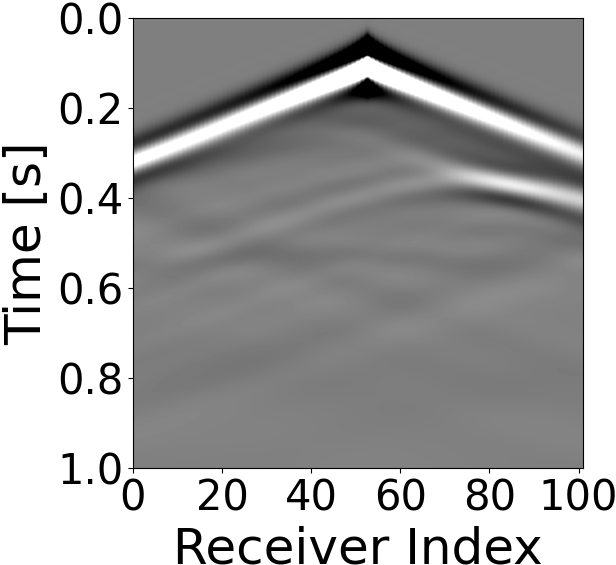
\includegraphics[width=\linewidth]{public/seismic_data}
%            \vspace{-7mm}
            \caption*{\raisebox{-2mm}{Seismic Data}}
%            \vspace{1mm}
        \end{minipage} &
        \begin{minipage}[b]{\linewidth}
            \centering
%            \vspace{1mm}
            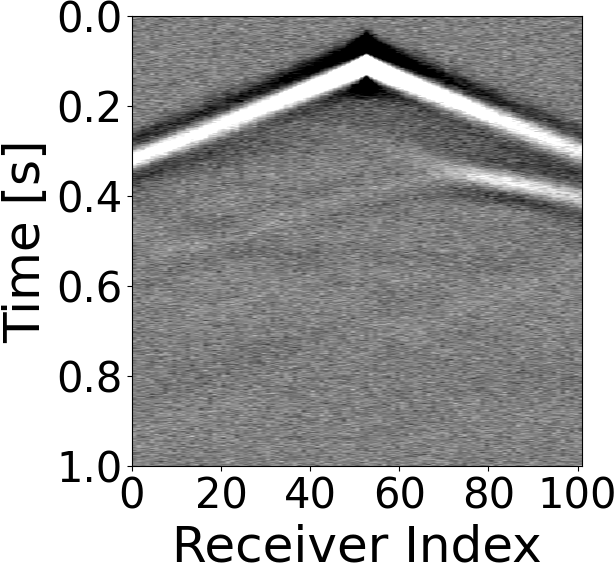
\includegraphics[width=\linewidth]{public/seismic_data_noisy}
%            \vspace{-7mm}
            \caption*{\raisebox{-2mm}{Noisy Seismic Data}}
%            \vspace{1mm}
        \end{minipage} &
        \hspace{-3mm}
        \multirow[t]{3}{*}{\raisebox{-5.8mm}{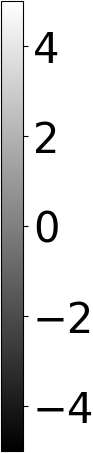
\includegraphics[height=24mm]{public/seismic-data-color-bar}}} \\
    \end{tabular}
%    \vspace{-4mm}
    \captionsetup{margin=1.3cm}
    \caption{The sinthesized seismic data \\ corresponding to a single source waveform.}
%    \vspace{-5mm}
    \label{fig:observed-seismic-data}
\end{figure}
